\subsection{Commande événementielle}
\begin{frame}[c]{Commande événementielle}
    \textbf{Principe \cite{astrom_event_2008} :}
    \begin{itemize}
        \item Alternative au contrôle périodique
        \item Actions déclenchées par événements
        \item Réduction des ressources
    \end{itemize}
    
    \vspace{0.3cm}
        
    \vfill
    
    \centering
    \begin{figure}
        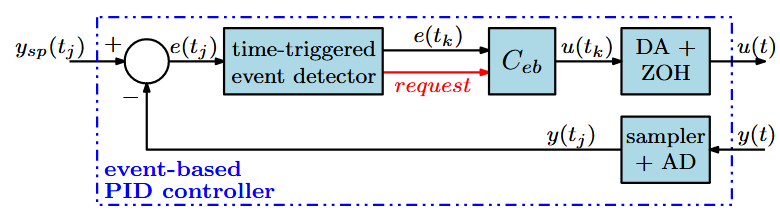
\includegraphics[width=0.7\textwidth]{3-etat-de-lart/pic/event-based-control.PNG}
        \caption{Schéma de commande événementielle \cite{durand_event-based_2015}}
    \end{figure}
\end{frame}


\begin{frame}[c]{Commande événementielle prédictive}
    \vfill
    \textbf{Objectif :} réduire les communications entre modules
    
    \vspace{0.3cm}
    
    \begin{columns}[T]
        \begin{column}{0.6\textwidth}
            \textbf{Principe :}
            \begin{itemize}
                \item Estimation de l'état des voisins
                \item Prédiction basée sur modèle dynamique
                \item Communication uniquement si écart > seuil
            \end{itemize}
            
        
        \end{column}
        \begin{column}{0.4\textwidth}
            \textbf{Avantages :}
            \begin{itemize}
                \item Réduction trafic réseau
                \item Adaptée aux grands systèmes
            \end{itemize}
            
            \vspace{0.3cm}
            \textbf{Inconvénients :}
            \begin{itemize}
                \item Complexité calcul
                \item Dépendance au modèle
            \end{itemize}
        \end{column}
    \end{columns}
    
    \vfill
\end{frame}

%\begin{frame}[c]{Défis de la commande événementielle}
%    \vfill
%    \textbf{Problèmes identifiés :}
%    
%    \vspace{0.3cm}
%    \textbf{1. Comportement Zeno \cite{yu_zeno_2021}}
%    \begin{itemize}
%        \item Nombre infini d'événements en temps fini
%        \item Solutions : borne temporelle minimale, seuils indépendants
%    \end{itemize}
%    
%    \vspace{0.3cm}
%    \textbf{2. Explosion de la partie intégrale}
%    \begin{itemize}
%        \item Accumulation pendant les périodes stables
%        \item Solutions : saturation du produit $h \cdot e$, facteur d'oubli
%    \end{itemize}
%    
%    \vspace{0.3cm}
%    \textbf{Applications réussies :}
%    \begin{itemize}
%        \item Quadricoptère avec motion capture
%        \item Réduction de 60\% des communications (microgrid)
%    \end{itemize}
%    \vfill
%\end{frame}
